\chapter{Study Areas}
\label{studyareas}

This study used agricultural areas in Kansas, USA for testing and verification of the phenological classification method and applied the classification method to Pellegrini, Santiago del Estero, Argentina to test its effectiveness in subtropical South America.


\section{Kansas, USA}
\label{studyareas:kansas}

The state of Kansas is one of the big agricultural producers of the U.S. As a plains state, it is relatively flat across much of its extent, making it well suited to large highly-mechanized agro-industrial operations. In 2012, the three most extensive crops in the state were wheat, corn, and soybeans (\autoref{table:kansas}), which are also the most abundant crops in Pellegrini, Argentina. Additionally, Kansas has been the focus of a number of previous studies into the use of MODIS time-series for crop classification \autocites{wardlow2002discriminating}{wardlow2005state-level}{wardlow2007analysis}{wardlow2008large-area}, and has a very detailed and easily-accessible crop cover dataset in the form of the USDA CDL. These factors make Kansas a natural choice for preliminary testing.

\begin{sstable}
  \centering
  \caption[Most extensive crops in Kansas, 2012.]{Most extensive crops in Kansas, 2012\\~\autocite[adapted from][]{usda2013kansascrops}}
  \label{table:kansas}
  \begin{tabu}{lcc}
    \toprule
    \textbf{Crop} & \textbf{Acreage (1,000 acres)} & \textbf{Production (1,000 units)} \\
    \midrule
    Wheat & 9,100 & 382,200 \\
    Corn & 3,950 & 379,200 \\
    Soy & 3,810 & 83,820 \\
    All Hay & 2,750 & 4,340 \\
    All Forage & 2,750 & 4,545 \\
    Sorghum & 2,100 & 81,900 \\      
    \bottomrule
  \end{tabu}
\end{sstable}

I delineated a small 100 MODIS pixel by 100 MODIS pixel study area just northwest of Wichita, Kansas. The communities of Valley Center, Sedgwick, and Halstead run linearly from the southeast corner to the northwest corner of the study site (\autoref{fig:KSstudysite}). I tested and verified the classification method in this area (see \autoref{appendix:testing} on \autopageref{appendix:testing} for a full overview of the Kansas testing), and I extracted the crop reference signatures used for the Argentina classification from this area. The typical planting dates for a variety of crops in this region are shown in \autoref{table:KSplantingdates}. I chose this specific study site because of the mix of land covers in the 2012 CDL reference (\autoref{fig:KScdl}) included corn, soy, sorghum, winter wheat, winter wheat and soy double crop, urban development, grassland, forest, and others.

\begin{ssfigure}
  \centering
  \includegraphics[width=\textwidth]{Graphics/KSstudysite.pdf}
  \caption[Kansas Study Site and the Communities of Halstead, Sedgwick, and Valley Center.]{Kansas Study Site and the Communities of Halstead,\\~Sedgwick, and Valley Center.}
  \label{fig:KSstudysite}
\end{ssfigure}

\begin{table}[b]
  \begin{Spacing}{1.0}
  \centering
  \caption[Kansas Study Site Planting Dates]{Kansas Study Site Planting Dates\\~\autocite[adapted from][]{shroyer1996kansas}}
  \label{table:KSplantingdates}
  \begin{tabu} to 4.5in {X[1,m,c]X[2,m,c]}
    \toprule
    \textbf{Crop} & \textbf{Planting Date Range} \\
    \midrule
    Wheat & \datenoyear{25}{9} to \datenoyear{20}{10} \\
    Triticale & \datenoyear{1}{9} to \datenoyear{25}{9} \\
    Winter Barley & \datenoyear{15}{9} to \datenoyear{10}{10} \\
    Spring Barley & \datenoyear{25}{2} to \datenoyear{15}{3} \\
    Spring Wheat & \datenoyear{25}{2} to \datenoyear{15}{3}\\
    Spring Oats & \datenoyear{25}{2} to \datenoyear{15}{3}\\
    Corn & \datenoyear{1}{4} to \datenoyear{10}{5} \\
    Sorghum & \datenoyear{15}{5} to \datenoyear{20}{6} \\
    Soybeans & \datenoyear{5}{5} to \datenoyear{10}{6} \\
    \bottomrule
  \end{tabu}
  \end{Spacing}
\end{table}


\begin{ssfigure}
  \centering
  \includegraphics[width=\textwidth]{Graphics/KScdl.pdf}
  \caption{2012 Kansas Study Site Crop Cover}
  \label{fig:KScdl}
  \medskip
  \small
  Corn, soy, and winter wheat are the predominate crops in this area of Kansas, in line with the top three crops of the state as a whole. The sorghum sample size is comparatively small, but I found few areas with higher concentrations of sorghum.
\end{ssfigure}

\section{Pellegrini, Santiago del Estero, Argentina}
\label{studyareas:pellegrini}

Santiago del Estero, a province in Northwest Argentina, has an area of 136,351 square kilometers, which is about the same size as the state of Arkansas. The population was about 874,000 in 2010 \autocite{estadistica-y-c2010a}. The entire province is classified within the \textit{Parque Chaqueño} (Chaco forest). Like the rest of Argentina forests, the remaining forested area has declined rapidly over the past fifteen years. During the period 1998 to 2002, 306,055 hectares were deforested \autocite{secretaria-de-a2007informe}. From 2006 through 2011, a further 701,030 hectares of forest were lost, 283,669 of which were after the enacting of the OTBN in March of 2009 \autocite{secreteria-de-a2012monitoreo}. Over both of these time periods, Santiago del Estero experienced the highest levels of deforestation in all of Argentina.

The Department of Pellegrini is an administrative area in the Northwest corner of the province of Santiago del Estero (\autoref{map:argentinaOverview}).\footnote{The Pellegrini boundary shapefile I obtained does not accurately reflect the bounds of the department on the ground. Particularly along the lengthy and straight northwestern edge, careful inspection reveals a lack of registration between the vector geometry and the obvious boundary visible in the background image. When investigating some of my sample points along the northern and southern edges, I got strange looks and comments about how this or that field was not within Pellegrini, my supposed study area. I want to acknowledge that I realize my study area is not actually the Department of Pellegrini proper, but an inaccurate representation as defined by a shapefile from the Internet. I use this inaccurate representation to ensure consistency, to allow repeatability, and to simplify spatial analysis.} The department has an area of 6,944 square kilometers, a size slightly larger than the state of Delaware. However, the 2010 population was only 20,514 \autocite{estadistica-y-c2010b}. The primary municipality of the department is Nueva Esperanza, with about 4,500 residents. \autoref{map:pellegriniCoverChange} shows Nueva Esperanza's location and the progression of deforestation in the department. Sometime between 1975 and 1993, an initial push for agricultural land began deforestation in the region. The frontier nature of Pellegrini seemed to limit further deforestation for some time. As can be seen from the satellite imagery, little changed between 1993 and 2001. And over the years 2001 to 2005, only 5,968 hectares were found to be deforested \autocite{volante2005analisis}. However, recent demand for land has amplified the rate of clearing. Over the period 2006 to 2011, over 75,000 hectares were cleared, a deforestation rate much higher than previously witnessed \autocite{secreteria-de-a2012monitoreo}. Some 39,480 of these hectares were cut after the enacting of the OTBN in 2009, when regulations should have slowed deforestation. Of the area cleared post-OTBN, 2,181 hectares were in red areas, the highest clearing of that designation in the nation. The vast majority of clearing was in yellow areas, totaling 29,796 hectares. Pellegrini’s total deforestation during the period 2006 to 2011 was not the highest in Santiago del Estero, as both Moreno Department and Alberdi Department had higher total deforestation. However, as a percent of total land area, Pellegrini’s deforestation occurred at a greater rate: 10.85 percent of Pellegrini’s land area was cleared versus 10.45 percent and 7.91 percent of Moreno and Alberdi, respectively.

\begin{ssfigure}
  \centering
  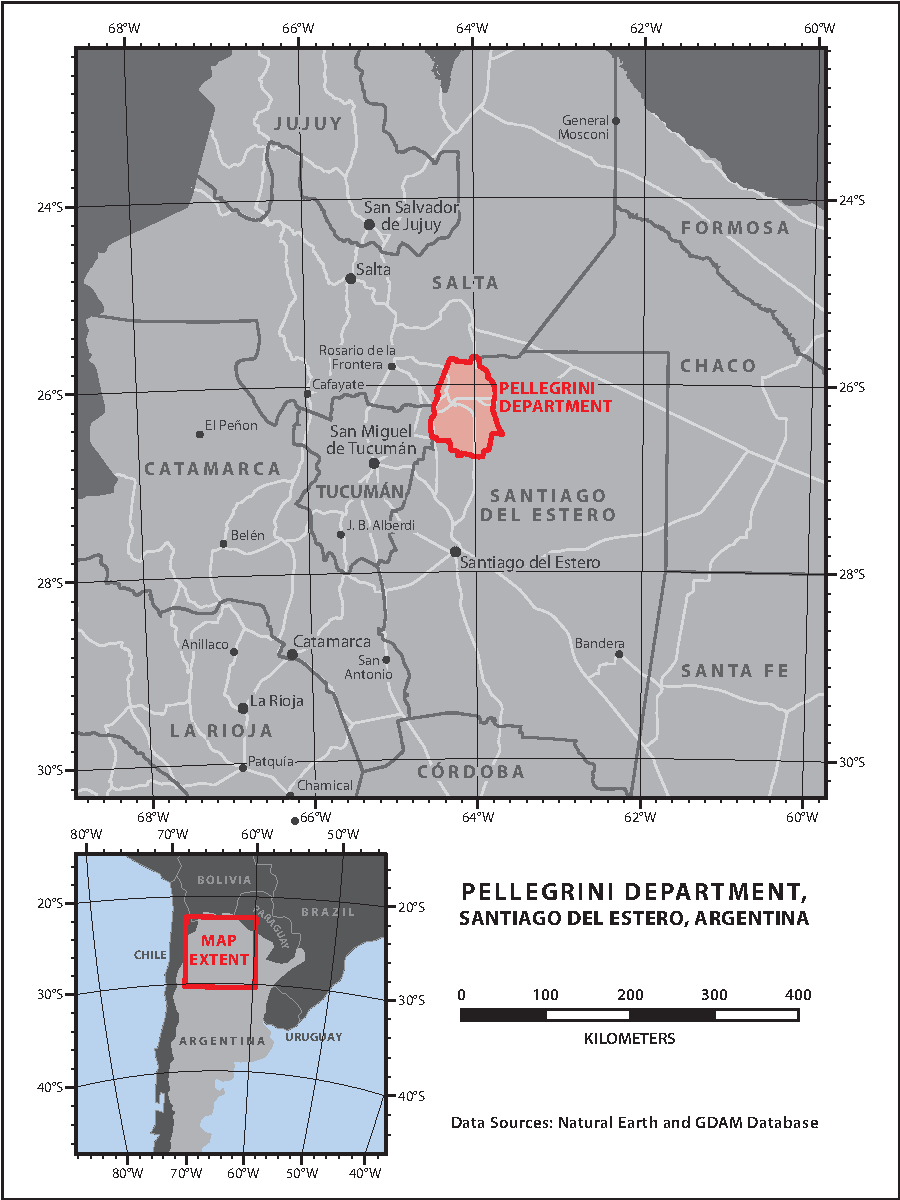
\includegraphics[width=\textwidth]{Graphics/argentinaOverview.pdf}
  \caption{The Department of Pellegrini and the Greater Northwest of Argentina}
  \label{map:argentinaOverview}
\end{ssfigure}

\begin{ssfigure}
  \centering
  \includegraphics[scale=.95]{Graphics/pellegrini75to14.pdf}
  \caption{Land Cover Change in Pellegrini from 1973 to 2014}
  \label{map:pellegriniCoverChange}
  \medskip
  \small
  These images show the progression of deforestation in Pellegrini. The lack of deforestation in the 1973-1975 composite is striking. As early as 1993, deforestation is visible, primarily in the Southwest near Tucumán Province. Little changed between 1993 and 2001, but by 2014 much more deforestation is visible throughout the entire area.
\end{ssfigure}

\textcite{volante2005analisis} found Pellegrini's primary summer crop over the years 2000 to 2005 to be soy, averaging about 40,000 hectares cultivated per year. Corn was the second most frequent crop, occupying about 7,500 hectares per year. \textit{Poroto}, a generic term for many types of common beans, was the third most popular, averaging a total cultivation of about 2,500 hectares per year. The primary winter crop was wheat, though cultivation varied wildly from less than 10,000 hectares in 2002 to over 31,000 hectares in 2004.

Specific planting dates for Pellegrini are not available, but crop calendars for Argentina as a whole do provide generalized information \autocites{agriculture-for2008foreign}{sacks2010crop}{soybean-and-cor2013argentina}. Corn is typically planted mid-September through the end of November, and sorghum follows about twenty days later. Soybeans are planted in two groups: early and late. Early soy is often planted mid-November through the end of December, while late soy follows the harvesting of winter wheat, typically between the beginning of December through the middle of January. Compared to \autoref{table:KSplantingdates}, these dates are approximately six months offset, congruent with Argentina's opposing location in the Southern Hemisphere. However, the Argentina planting date ranges are noticeably longer than those in Kansas.

%Harvesting of both corn and sorghum occurs from the end of March through the middle of June. Early soy is harvested from the end of March through the middle of May while late soy is not ready until the end of April, taking until mid-June to be completely harvested.